
\documentclass[aspectratio=169]{beamer}
\usepackage[spanish]{babel}
\usepackage[utf8x]{inputenx}
\usepackage{multicol} % indice en 2 columnas
\usepackage{subfig}
\usepackage{tikz-timing}[2009/05/15]
\usepackage{enumerate} % enumerados
\usepackage{wrapfig} %preámbulo
%\usepackage{pstricks}
\usepackage{textpos}

\usetheme{CambridgeUS}
\usecolortheme{seahorse}
%\useoutertheme{shadow}
%\useinnertheme{circles}




\title[GraspJ]{GraspJ - GPU-Run Analysis for STORM and PALM in ImageJ}

\subtitle{AFIB - ICFO}

\author[Ismael Benito]{\bigskip \small Ismael Benito Altamirano}
\date[AFIB - ICFO]{\small \today}

\AtBeginSection{
\begin{frame}
  \frametitle{Index}
  \tableofcontents[currentsection] 
\end{frame}
}

\begin{document}

%\begin{frame}
%\maketitle
%\end{frame}

\addtobeamertemplate{frametitle}{}{%
\begin{textblock*}{110mm}(.65\textwidth,-1,25cm)

\includegraphics[height=1.5cm]{./images/logos.png}
\end{textblock*}}

\frame{\titlepage}

\begin{frame}
  \frametitle{Index}
  \tableofcontents
\end{frame}

\section{Introducing GraspJ}

\begin{frame}
\frametitle{Introducing GraspJ}

\textbf{GraspJ - GPU-Run Analysis for STORM and PALM in ImageJ}


\end{frame}

\subsection{Java \& OpenCL}

\begin{frame}
 
\frametitle{Java \& OpenCL}
 
\end{frame}





\section{GraspJ Views}

\begin{frame}

\begin{figure}[h!]
    \centering	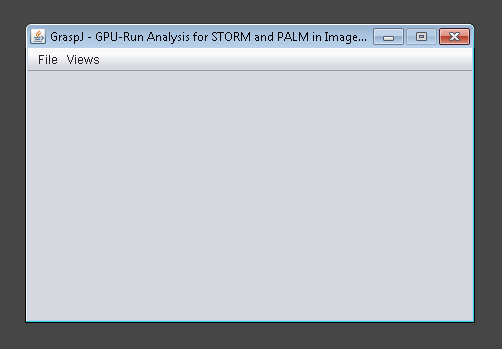
\includegraphics[width=0.4\textwidth]{./images/graspj.png} 
    \caption{}
    \label{fig:graspj}
    \end{figure} 
 
\end{frame}

\subsection{Workflow Wizard View}

\begin{frame}
 
 \begin{figure}[h!]
    \centering	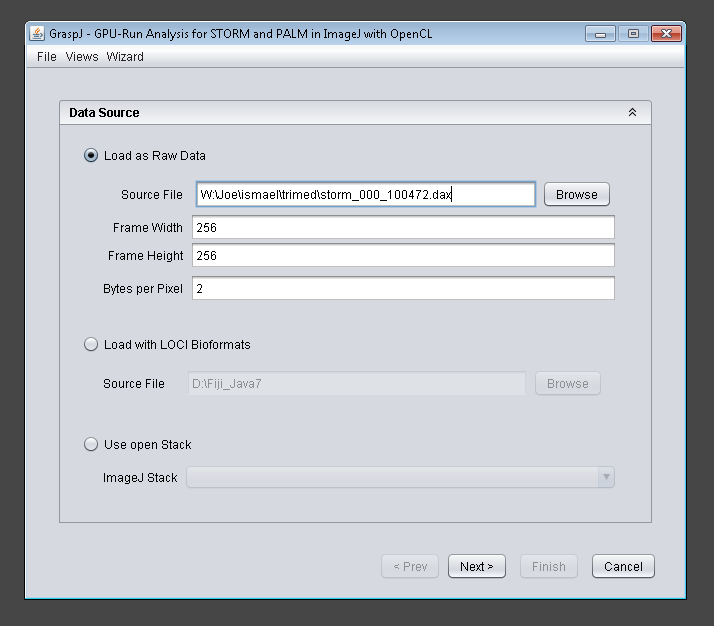
\includegraphics[width=0.4\textwidth]{./images/graspj_workflow1.png} 
    \caption{}
    \label{fig:workflow}
    \end{figure} 
 
\end{frame}


\begin{frame}
 
 \begin{figure}[h!]
    \centering	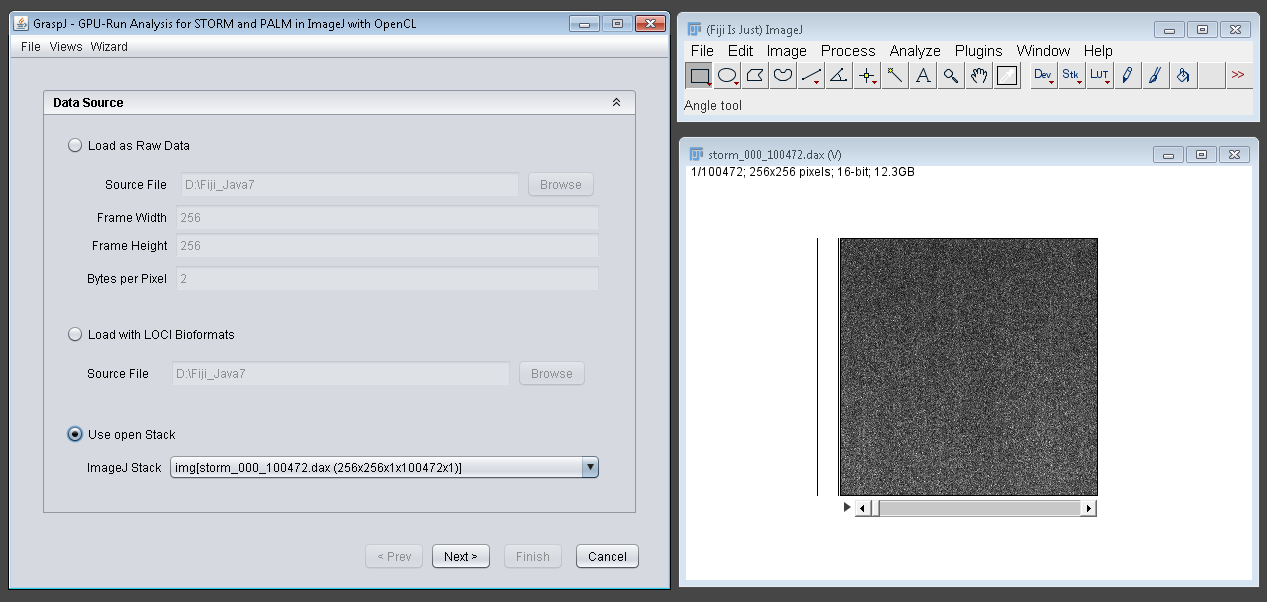
\includegraphics[width=0.4\textwidth]{./images/graspj_workflow2.png} 
    \caption{}
    \label{fig:workflow2}
    \end{figure} 
 
\end{frame}

\begin{frame}
 
 \begin{figure}[h!]
    \centering	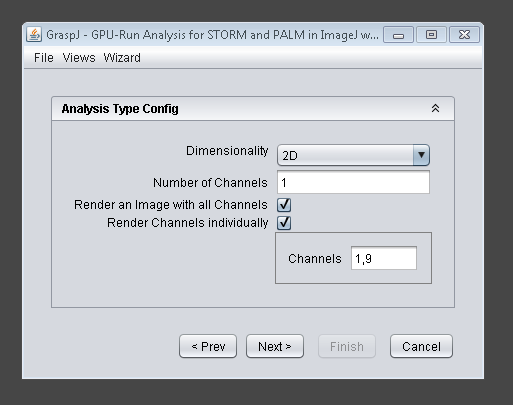
\includegraphics[width=0.4\textwidth]{./images/graspj_workflow3.png} 
    \caption{}
    \label{fig:workflow3}
    \end{figure} 
 
\end{frame}

\begin{frame}
 
 \begin{figure}[h!]
    \centering	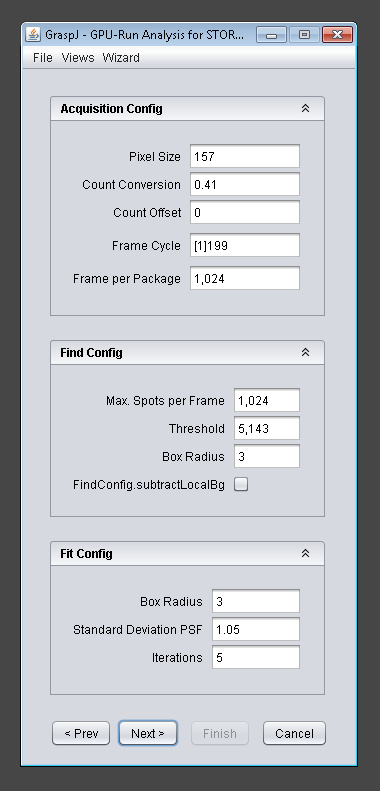
\includegraphics[width=0.4\textwidth]{./images/graspj_workflow4.png} 
    \caption{}
    \label{fig:workflow4}
    \end{figure} 
 
\end{frame}


\subsection{Workflow View}

\begin{frame}
 
 \begin{figure}[h!]
    \centering	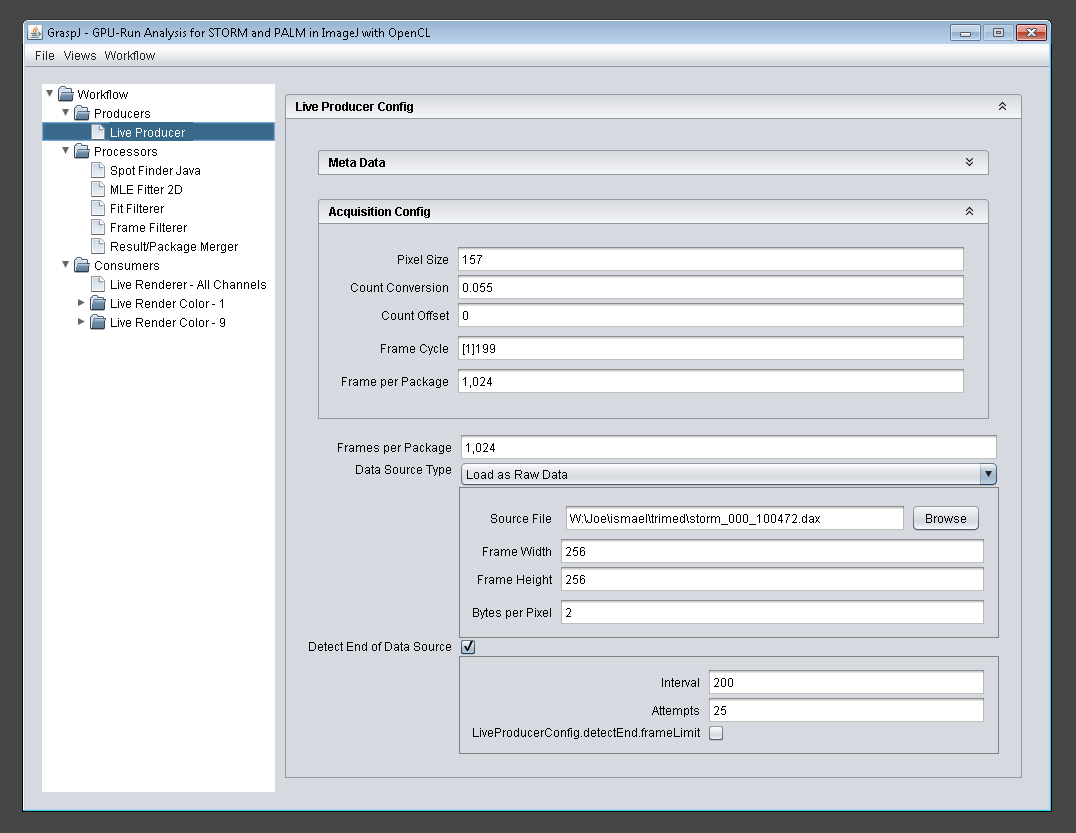
\includegraphics[width=0.4\textwidth]{./images/graspj_workflow5.png} 
    \caption{}
    \label{fig:workflow5}
    \end{figure} 
 
\end{frame}

\subsection{Running Analysis View}

\begin{frame}
 
 \begin{figure}[h!]
    \centering	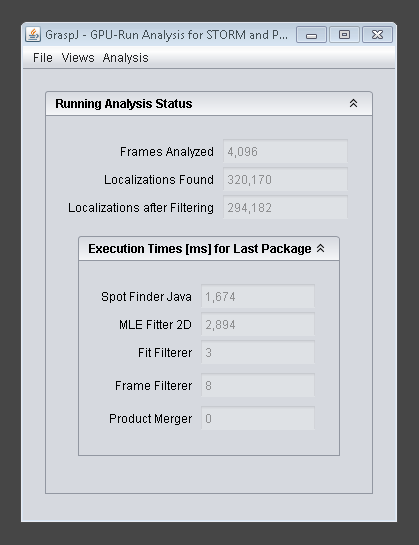
\includegraphics[width=0.4\textwidth]{./images/graspj_running1.png} 
    \caption{}
    \label{fig:running}
    \end{figure} 
 
\end{frame}

\subsection{Results View}
\begin{frame}
 
 \begin{figure}[h!]
    \centering	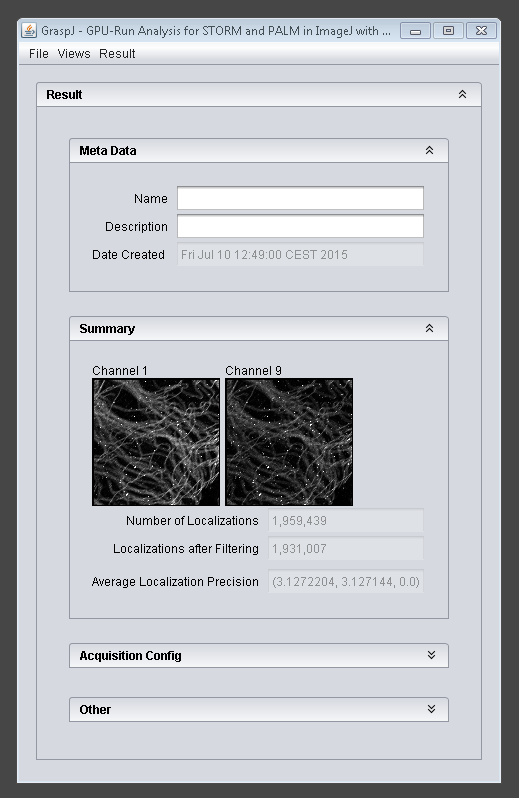
\includegraphics[width=0.4\textwidth]{./images/graspj_results1.png} 
    \caption{}
    \label{fig:results1}
    \end{figure} 
 
\end{frame}

\begin{frame}
 
 \begin{figure}[h!]
    \centering	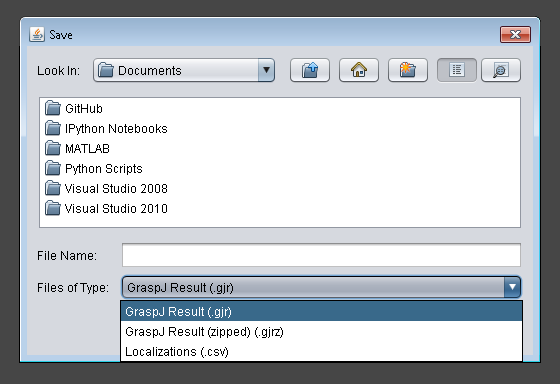
\includegraphics[width=0.4\textwidth]{./images/graspj_results2.png} 
    \caption{}
    \label{fig:results2}
    \end{figure} 
 
\end{frame}

\section{Errors}

\section{DAOSTORM}





\end{document}